This section will be discussing on the intrinsic value and market of an equity, particularly on stocks 

\begin{multicols}{2}
    
\subsection{intrinsic Value}
Value $V$ based on a fundamental analysis of a company's current assets and future prospects. It is the discounted value of the cash that can be taken out of a business during its remaining life. 

\subsection{Market Value}
Value $P$ based on observed market prices and shares outstanding.

\subsection{Dividend Discount Model (DDM)}
Equity's value is equal to the discounted value of all future dividends.
\begin{gather*}
    \begin{split}
        V_0 = P_0 &= \frac{E(D_1)}{1+R}+\frac{E(P_1)}{1+R}\\
        &= \frac{E(D_1)}{1+R} + \frac{E(\frac{E(D_2)}{1+R}+\frac{E(P_2)}{1+R})}{1+R}\\
        &= \frac{E(D_1)}{1+R}+\frac{E(D_2)+E(P_2)}{(1+R)^2}\\
        &= \frac{E(D_1)}{1+R} + \frac{E(D_2)}{(1+R)^2} + \frac{E(D_3)}{(1+R)^3} + \cdots
    \end{split}
\end{gather*}
In order to price a equity from its dividends, we first need to find out how to evaluate a company's dividend.

\subsection{Expected Dividend}
\subsubsection{Dividend Payout Ratio}
Ratio $d$ is equal to the expected share of earnings that will be paid out as a \underline{\textbf{dividend}}.
\begin{gather*}
    \boxed{D_t = d_t\times E_t}
\end{gather*}

\subsubsection{Earnings-Retention Ratio}
Ratio $b$ is equal to the expected share of earnings that will be \underline{\textbf{reinvested}}.
\begin{gather*}
    I_t = b_t\times E_t = (1-d_t)E_t
\end{gather*}
if the retained earnings fund new projects with return $ri$. the expected return can then expressed as
\begin{gather*}
    E_{t+1} = E_t + I_t\times ri_{t+1} = E_t+b_t\times E_t\times ri_{t+1}\\
    \boxed{g_{t+1}=\frac{E_{t+1}-E_t}{E_t} = b_t\times ri_{t+1}}
\end{gather*}
This leads to The \underline{\textbf{Growth Rate of Earnings}}:

\subsection{DDM Analysis}
\subsubsection{D constant}
Suppose that the dividends are \underline{\textbf{constant}}, i.e. $E(D_1) = D_0, E(D_2) = D_0...$
\begin{gather*}
    \begin{split}
        V_0 &= \frac{E(D_1)}{1+R} + \frac{E(D_2)}{(1+R)^2}+\cdots\\
        &= \frac{D_0}{1+R} + \frac{D_0}{(1+R)^2}+\cdots = \boxed{\frac{D_0}{R}}
    \end{split}
\end{gather*}
\subsubsection{D grow at rate g}
Suppose now the \underline{\textbf{dividends grow}} at a rate g, i.e. $E(D_1) = (1+g)D_0$, $E(D_2) = (1+g)^2D_0$
\begin{gather*}
    \begin{split}
        V_0 &= \frac{D_0(1+g)}{1+R}+\frac{D_0(1+g)^2}{(1+R)^2}+\cdots\\
        &= \frac{D_0(1+g)}{R-g} = \boxed{\frac{(1-b)E(E_1)}{R-g}}
    \end{split}
\end{gather*}
This is also called the \underline{\textbf{Gordon Growth Model}}\par 

From the table below, the amount of investment increases from left to right, and price adjust accordingly. If the return on new investment is exactly $\boxed{\textbf{equal}}$ to the \textcolor{red}{\textbf{CAPM implied return}}, the things I'm investing in are compensating me exactly as well as the stock should be compensating me, so the price will remain unchanged\par 

If the new investment return is $\boxed{\textbf{lower}}$ than my CAPM implied return, that means I'm investing into something bad that doesn't gives me enough return, therefore, the \underline{\textbf{stock price must decrease}} in order to \textbf{increase} the expected return. 

Likewise, if my new investment return is $\boxed{\textbf{higher}}$ than my CAPM implied return, than the stock \underline{\textbf{price must increase}} in order to \textbf{decrease} the expected return.\footnote{a stock with a very high price will require a larger dollar change in price to achieve the same percentage return as a stock with a very low price, resulting in a lower percentage return for the higher-priced stock. E.g. Stock A is priced at \$500 per share and Stock B is priced at \$50 per share. If both stocks increase in price by \$50 per share over a period of time, Stock A would have a 10\% return (\$50 / \$500), while Stock B would have a 100\% return (\$50 / \$50)}


\subsection{Two stage valuation}
If a company dividends grow at different rates over time, i.e. first stage at rate $g_1$, second stage $g_2$ 
\begin{gather*}
    V_0 = \sum_{t =1}^{T}\frac{D_0(1+g_1)^t}{(1+R)^t} + \frac{D_T(1+g_2)}{(R-g_2)(1+R)^T}
\end{gather*}

\subsection{Valuation Ratio}
\subsubsection{Price-dividend ratio}
\begin{gather*}
    \frac{P}{D} = \frac{1+g}{R-g}
\end{gather*}

\subsubsection{Price-earnings ratio}
\begin{gather*}
    \frac{P}{E} = \frac{(1+g)(1-b)}{R-g}
\end{gather*}

\end{multicols}

\begin{figure}[H]
    \centering 
    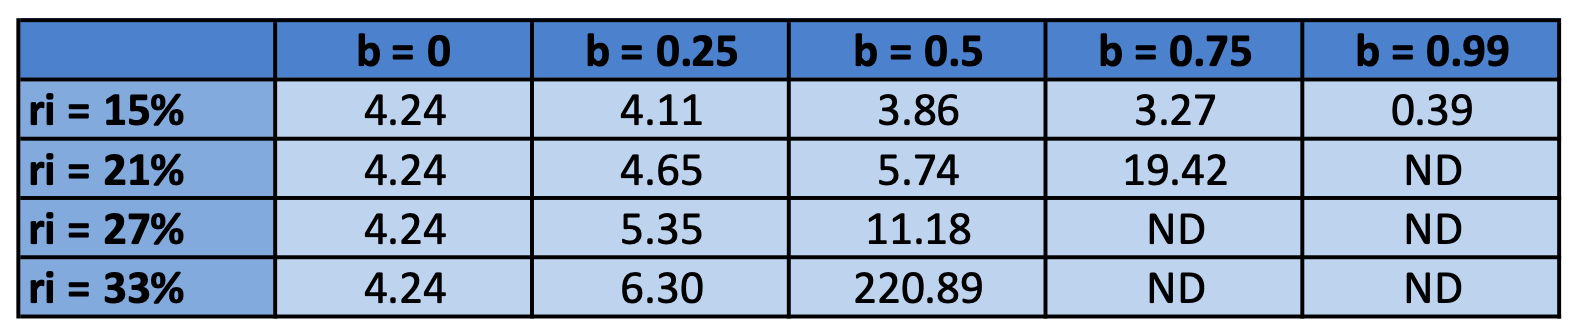
\includegraphics[width =0.7\textwidth]{Figure/table.png}
\end{figure}


